\documentclass[12pt,a4paper]{report}

% --- Paquets bàsics ---
\usepackage[catalan]{babel}
\usepackage[utf8]{inputenc}
\usepackage[T1]{fontenc}
\usepackage{lmodern}
\usepackage{geometry}
\usepackage{setspace}
\usepackage{graphicx}
\usepackage[hidelinks]{hyperref}
\usepackage{amsmath}
\usepackage{amsfonts}
\usepackage{amssymb}
\usepackage{float}
\usepackage{listings}
\usepackage{xcolor}
\usepackage{caption}
\begin{document}

\chapter{Transelevadores i sistemes AS/RS}


\section{Què és un transelevador}


Un transelevador \cite{transelevador_info} és un equip automàtic de manipulació de materials utilitzat en sistemes d'emmagatzematge automatitzat (AS/RS), dissenyat per transportar, emmagatzemar i recuperar unitats de càrrega dins d'estanteries industrials.

Aquest sistema es desplaça habitualment per un passadís mitjançant rails, permetent el moviment en diferents direccions per accedir a qualsevol ubicació del magatzem. La seva funció principal és automatitzar les operacions logístiques, reduint la intervenció humana i augmentant l'eficiència del sistema.

Els transelevadors (\ref{fig:transelevador1}) podden treballar de forma completament automàtica, controlats per sistemes informàtics, o bé en mode manual en funció de l'aplicació.

\begin{figure}[H]
    \centering
    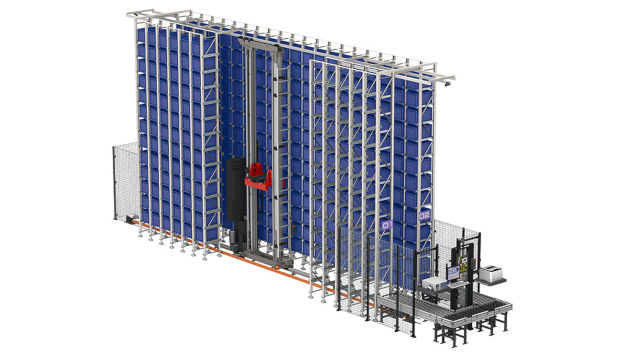
\includegraphics[width=0.7\linewidth]{images/miniload-asrs.jpg}
    \caption{Sistema d'emmagatzematge automatitzat (AS/RS) amb transelevador tipus miniload \cite{asrs_daifuku}.}
    \label{fig:transelevador1}
\end{figure}


\section{Contextos d'aplicació dels sistemes AS/RS}
Els sistemes AS/RS (Automated Storage and Retrieval Systems) són sistemes d'emmagatzematge automatitzat controlats per ordinador, utilitzats en entorns industrials i logístics per gestionar el flux de materials de manera eficient.

Aquests sistemes s'apliquen principalment en dos grans àmbits \cite{asrs_daifuku}:

\begin{itemize}
    \item \textbf{Indústria de fabricació}:
    \begin{itemize}
        \item Emmagatzematge de matèries primeres
        \item Subministrament de components a línies de producció
        \item Gestió de productes en procés (buffers)
        \item Emmagatzematge de producte final
    \end{itemize}

    \item \textbf{Logística i distribució}:
    \begin{itemize}
        \item Emmagatzematge temporal de productes
        \item Preparació de comandes
        \item Classificació i agrupació de mercaderies per a enviament
    \end{itemize}
\end{itemize}

Els AS/RS permeten un ús eficient de l'espai vertical del magatzem, incrementant la densitat d'emmagatzematge i millorant la gestió de l'inventari.

A més, contribueixen a la reducció de costos laborals, a la millora de la seguretat i a una major precisió en les operacions logístiques.



\section{Funcionament del transelevador}

El funcionament d'un transelevador \cite{transelevador_info} basa en un sistema automatitzat capaç de realitzar moviments coordinats per accedir a qualsevol posició dins del magatzem.

Aquest sistema opera principalment mitjançant tres moviments:

\begin{itemize}
    \item \textbf{Moviment longitudinal}: desplaçament al llarg del passadís sobre rails.
    \item \textbf{Moviment vertical}: elevació i descens de la càrrega mitjançant el màstil.
    \item \textbf{Moviment de càrrega}: introducció o extracció de la unitat de càrrega dins de l'estanteria.
\end{itemize}


En sistemes més avançats, els transelevadors es coordinen amb altres equips com cintes transportadores o sistemes de llançadora, integrant-se en un sistema logístic completament automatitzat.

Aquests sistemes poden operar amb diferents tipus de càrrega, permetent adaptar el sistema a diferents necessitats industrials:

\begin{itemize}
    \item \textbf{Càrrega unitària}: palets o elements pesants.
    \item \textbf{Minicàrrega}: caixes, contenidors o productes lleugers.
\end{itemize}

\section{Parts principals d'un transelevador}

Un transelevador està format per diferents subsistemes mecànics i electrònics que permeten el seu funcionament automatitzat dins del magatzem (Figura \ref{fig:parts_transelevador}).

Entre els principals elements \cite{transelevador_info} que el componen destaquen:

\begin{itemize}
    \item \textbf{Sistema de presa de càrrega}: habitualment una pinça o plataforma elevadora que permet la manipulació de la unitat de càrrega dins de les estanteries.

    \item \textbf{Sistema de sensors}: conjunt de dispositius encarregats de detectar la posició, presència de càrrega i estat del sistema, essencials per al control automàtic.

    \item \textbf{Sistemes d'accionament}: motors elèctrics que permeten els moviments principals del transelevador(vertical, horitzonatl i transversal):

    \item \textbf{Sistema de manipulació extensible}: mecanismes que permeten introduir i extreure la càrrega de les estanteries.

    \item \textbf{Estructura mecànica}: formada per màstil o columna, xassís superior i inferior, i sistemes de guia sobre rails.

    \item \textbf{Unitat d'elevació}: inclou la cuna o plataforma elevadora, motor d'elevació i sistemes de seguretat associats.

    \item \textbf{Unitat de traslació}: permet el moviment longitudinal mitjançant rodes sobre rails, amb sistemes anti-descarrilament.

    \item \textbf{Sistema elèctric}: armari elèctric, sistemes d'alimentació i protecció.

    \item \textbf{Sistema de control}: pot ser manual (cabina d'operador) o automàtic mitjançant sistemes basats en microprocessadors.

    \item \textbf{Punt de comandament}: pot ser embarcat, remot o d'emergència.
\end{itemize}

Aquests sistemes treballen conjuntament per permetre el moviment eficient de càrregues en passadissos estrets i a gran altura.


\begin{figure}[H]
    \centering
    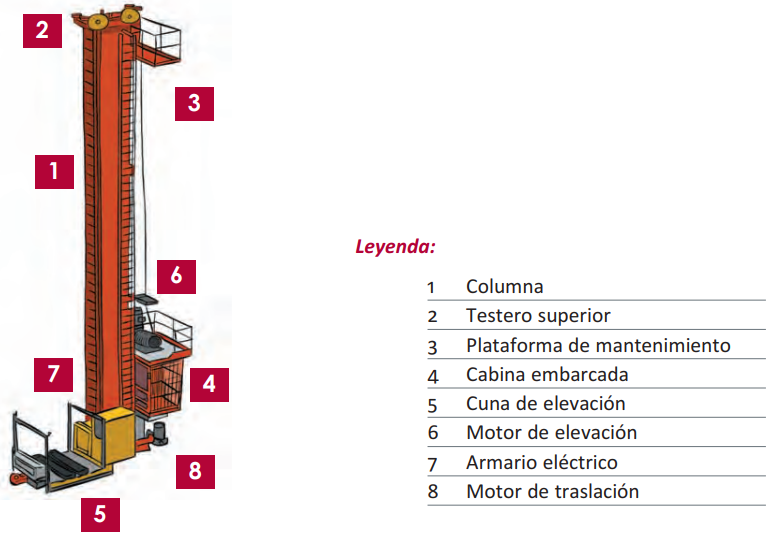
\includegraphics[width=0.5\linewidth]{images/parts_trans.PNG}
    \caption{Parts principals d'un transelevador industrial \cite{manual_logistica}.}
    \label{fig:parts_transelevador}
\end{figure}

\section{Normativa i estanteries en sistemes AS/RS}

Els transelevadors són equips industrials automatitzats que han de complir diferents normatives de seguretat i disseny, tant a nivell europeu com estatal.

Les principals normatives aplicables \cite{manual_logistica} són:

\begin{itemize}
    \item \textbf{Directiva 2006/42/CE}: regula els requisits de seguretat en el disseny de màquines.
    \item \textbf{Reial Decret 1215/1997}: estableix les condicions de seguretat en l'ús d'equips de treball.
    \item \textbf{UNE-EN 528}: norma específica per a transelevadors.
    \item \textbf{UNE-EN 1090-1}: relacionada amb estructures metàl·liques.
\end{itemize}

A més, aquests sistemes requereixen documentació tècnica obligatòria, com el manual d'instruccions, certificat CE, resultats d'assajos i registres d'inspecció.

\subsection{Norma UNE-EN 15620 i classificació d'estanteries}

El disseny del sistema també depèn de les estanteries utilitzades \cite{rack_estanterias_norma}. La norma \textbf{UNE-EN 15620} defineix toleràncies i precisió en sistemes d'emmagatzematge.

Segons aquesta norma, les estanteries es classifiquen en:

\begin{itemize}
    \item \textbf{Classe 100}: transelevadors automàtics en instal·lacions estàndard (altura inferior a 18m).
    \item \textbf{Classe 200}: major precisió amb sistemes de posicionament comparat amb la classe 100.
    \item \textbf{Classe 300A}: passadissos molt estrets amb operació guiada.
    \item \textbf{Classe 300B}: similar però amb menor assistència.
    \item \textbf{Classe 400}: sistemes manuals amb carretons convencionals.
\end{itemize}

Aquesta classificació és clau per determinar el nivell d'automatització i precisió del sistema.

\begin{figure}[H]
    \centering
    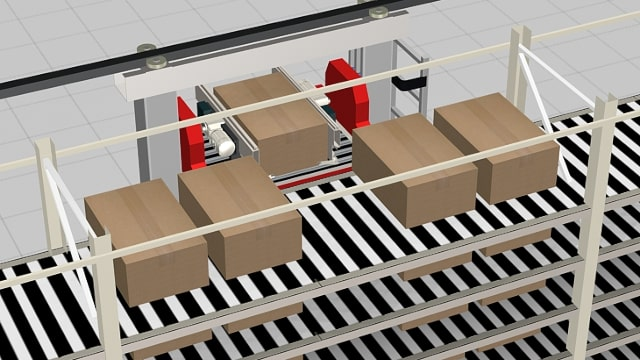
\includegraphics[width=0.56\linewidth]{images/shelving-rack.jpg}
    \caption{Exemple d'estanteries per a sistemes automatitzats tipus miniload. Font: Daifuku.}
\end{figure}


\section{Seguretat en els transelevadors}
Els transelevadors operen en entorns automatitzats amb moviments d'alta velocitat i manipulació de càrregues, fet que implica riscos que han de ser controlats adequadament.

Els principals riscos associats inclouen:
\begin{itemize}
    \item Aplastament per impacte amb estructures
    \item Caiguda de càrregues
    \item Contactes elèctric
    \item Caigudes en operacions de manteniment
    \item Errors de control del sistema
\end{itemize}

Per minimitzar aquests riscos \cite{manual_logistica}, els sistemes incorporen diferents mesures de seguretat com ara \textbf{parades d'emergència} accessibles, \textbf{control d'accés} mitjançant enclavaments, \textbf{sensors} de seguretat i finals de carrera, així com \textbf{sistemes anti-caiguda} i \textbf{reguladors de velocitat}.

A nivell de disseny, també s'integren dispositius com sistemes antidescarrilament, frenada automàtica en cas de fallada d'energia i limitadors de recorregut i velocitat.

Finalment, el sistema de control evita canvis de mode no autoritzats i garanteix la coherència entre accessos i comandaments, assegurant un funcionament segur en tot moment.


\section{Condicions d'ús i manteniment}

Els transelevadors són equips sotmesos a un ús intensiu i continu, especialment en sistemes automatitzats, per la qual cosa requereixen un manteniment adequat i un control estricte del seu estat.

Segons la normativa aplicable \cite{manual_logistica}, aquests equips han de sotmetre's a inspeccions periòdiques realitzades per personal autoritzat. Entre els aspectes clau destaquen:

\begin{itemize}
    \item Inspeccions periòdiques segons el manual del fabricant
    \item Revisió anual d'almenys el 20\% de la instal·lació
    \item Inspecció completa cada 5 anys
    \item Assajos funcionals amb càrrega nominal i addicional
\end{itemize}

El manteniment inclou:

\begin{itemize}
    \item Substitució preventiva de components
    \item Lubricació d'elements mecànics
    \item Control de sistemes de seguretat
    \item Verificació del correcte funcionament dels sensors i actuadors
\end{itemize}

Pel que fa a les condicions d'ús:

\begin{itemize}
    \item L'operador ha de ser major d'edat, format i autoritzat
    \item S'ha de registrar qualsevol incidència o avaria
    \item No es permet l'accés a persones als passadissos durant el funcionament
    \item S'han de seguir protocols estrictes en operacions de manteniment
\end{itemize}

Finalment, és obligatori disposar de procediments d'emergència i realitzar simulacres periòdics per garantir una resposta adequada davant possibles fallades del sistema.

\section{Relació del sistema desenvolupat amb els sistemes AS/RS i transelevadors}

El sistema desenvolupat en aquest treball es pot classificar conceptualment com un sistema AS/RS (Automated Storage and Retrieval System) \cite{asrs_daifuku}, ja que implementa una gestió automatitzada del flux de materials, incloent transport, emmagatzematge i evacuació de peces.

Un dels elements clau és la utilització de transelevadors, que reprodueixen el comportament típic d'aquests equips industrials mitjançant moviments coordinats en eixos vertical i horitzontal per posicionar càrregues en diferents nivells d'estanteria.

A més, el sistema integra característiques pròpies dels AS/RS reals, com ara l'automatització del procés, el control de posició mitjançant sensors i la gestió estructurada de l'emmagatzematge.

Tot i això, cal destacar que es tracta d'un model simplificat respecte a instal·lacions industrials reals (Figura \ref{fig:comparacion_asrs}). Per exemple, no s'inclouen aspectes com la gestió multi-passadís, sistemes redundants, optimització avançada de rutes o integració amb sistemes ERP.

Una descripció detallada del funcionament i de la implementació del sistema es presenta al capítol de disseny CITAR CAPITULO.

\begin{figure}[H]
\centering

\begin{minipage}{0.42\textwidth}
    \centering
    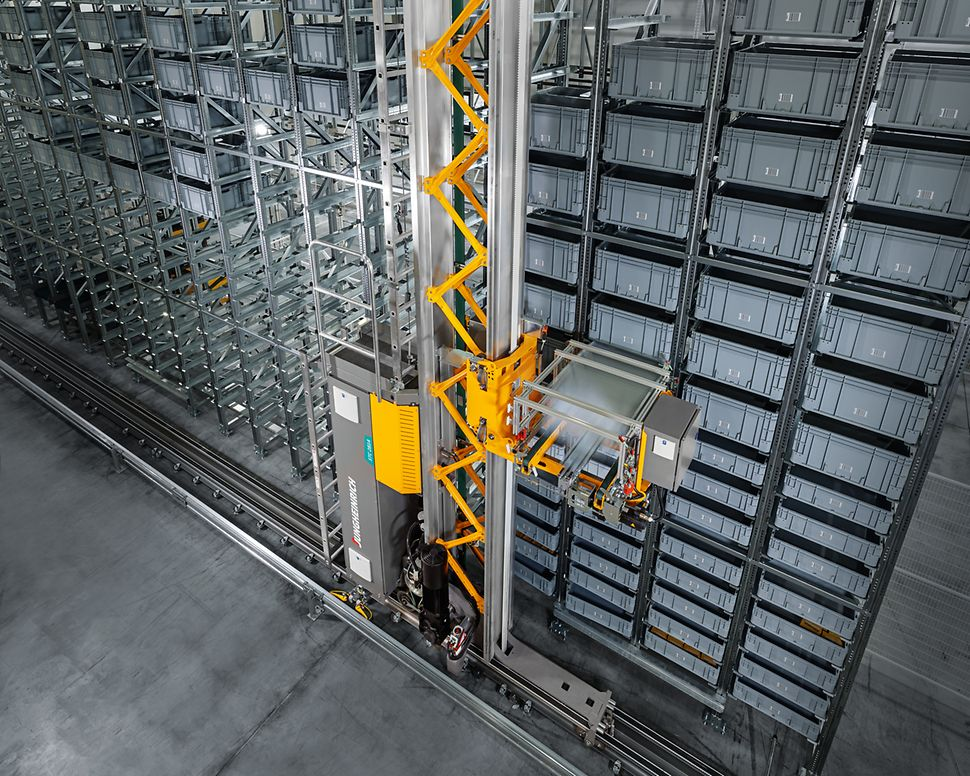
\includegraphics[width=\linewidth]{images/stage-miniload.jpg}
    \caption*{Sistema AS/RS industrial amb transelevador real \cite{transelevadores_jungheinrich}}  
\end{minipage}
\hfill
\begin{minipage}{0.42\textwidth}
    \centering
    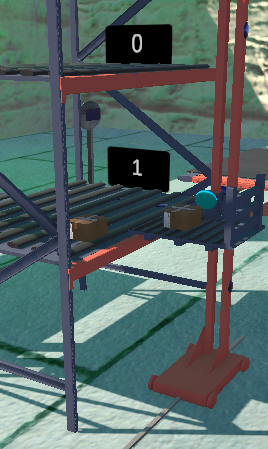
\includegraphics[width=0.65\linewidth]{images/unity_transelevador.png}
    \caption*{Model desenvolupat en Unity del sistema implementat}
\end{minipage}

\caption{Comparació entre un sistema AS/RS real i el model desenvolupat en aquest treball}
\label{fig:comparacion_asrs}
\end{figure}

\end{document}


https://inspecciontecnicadeestanterias.com/clases-de-estanterias-segun-la-norma-une-en-15620/
https://prevencion.fremap.es/Buenas%20prcticas/LIB.021%20-%20Guia%20seg.%20almacenam.%20y%20manejo%20cargas.pdf
https://szkolenia-udt.pl/es/publicaciones/derechos-tdt-ukladder/
https://www.daifuku.com/es/solution/intralogistics/products/automated-warehouse/types-features/
%https://www.jungheinrich.es/automatizaci%C3%B3n-y-sistemas/almacen-automatico-de-piezas-pequenas/transelevadores-piezas-peque%C3%B1as}